\chapter{Modellbildung} \label{ch_Modellbildung}
Die Modellbildung hat das Ziel das Zusammenspiel des Heliostatenfeldes und des Receivers am Solarturm in Jülich zu beschreiben.
Zu diesem Zweck wird das in Kapitel \ref{sec_Ausgangszustand} vorgestellte Modell eines Absorbercups um die Lüftungsdynamik im Receiver auf ein thermisches Teilmodell erweitert.
Darüber hinaus wird ein optisches Teilmodell zur Beschreibung der solaren Einstrahlung, der Heliostaten und deren Brennflecken auf dem Receiver eingeführt.
Abschließend wird die Modellbildung durch die Kopplung der beiden Teilsysteme vervollständigt.

\section{Thermisches Teilmodell} \label{sec_thermischesModell}
Zur Regelung des Massenstroms im Receiver müssen die Gebläse und Ventile im Luftkreislauf angesteuert werden.
Gemäß \cite[S.10ff]{DissGall} existieren zwei Gebläse/Ventil-Kombinationen, durch die der Luftdurchsatz im Receiver, am Wärmespeicher und am Dampfkraftprozess aufgeteilt wird.
Jede der Gebläse/Ventil-Kombinationen wird mittels eines Einstellwertes angesteuert.
In einer integrierten zweistufigen Regelung werden abhängig von diesem Einstellwert Ventilstellung und Gebläsedrehzahl angepasst, um einen gewünschten Luftmassenstrom zu erreichen.
Im Rahmen dieser Arbeit wird lediglich die Gebläse/Ventil-Kombination geregelt, die den Massenstrom im Receiver einstellt, da die weitere Verwendung dieser Luft zur Stromerzeugung oder Speicherung nicht betrachtet wird.

\subsection{Analyse der Lüftungsdynamik}
Durch die Vereinigung von Ventil und Gebläse entsteht bei einem Sprung des Einstellwertes eine gedämpft schwingende Anpassung des Luftstroms mit Verzögerung zweiter Ordnung.
Dieses Verhalten zeigt die in Abbildung \ref{fig_LuftstromSolarturm} dargestellte Messung am Solarturm vom 07.08.2022.
Auf der rechten Achse ist der dimensionslose Einstellwert der Gebläse/Ventil-Kombination erkennbar, während links der zugehörige Massenstrom aufgetragen ist.
Es ist ersichtlich, dass die Änderung des Luftmassenstroms um 12:20 Uhr Störungen unterlag. \newpage

\begin{figure}[h!]
    \centering
    \setlength{\fboxsep}{1pt}
    \setlength{\fboxrule}{1pt}
    \fbox{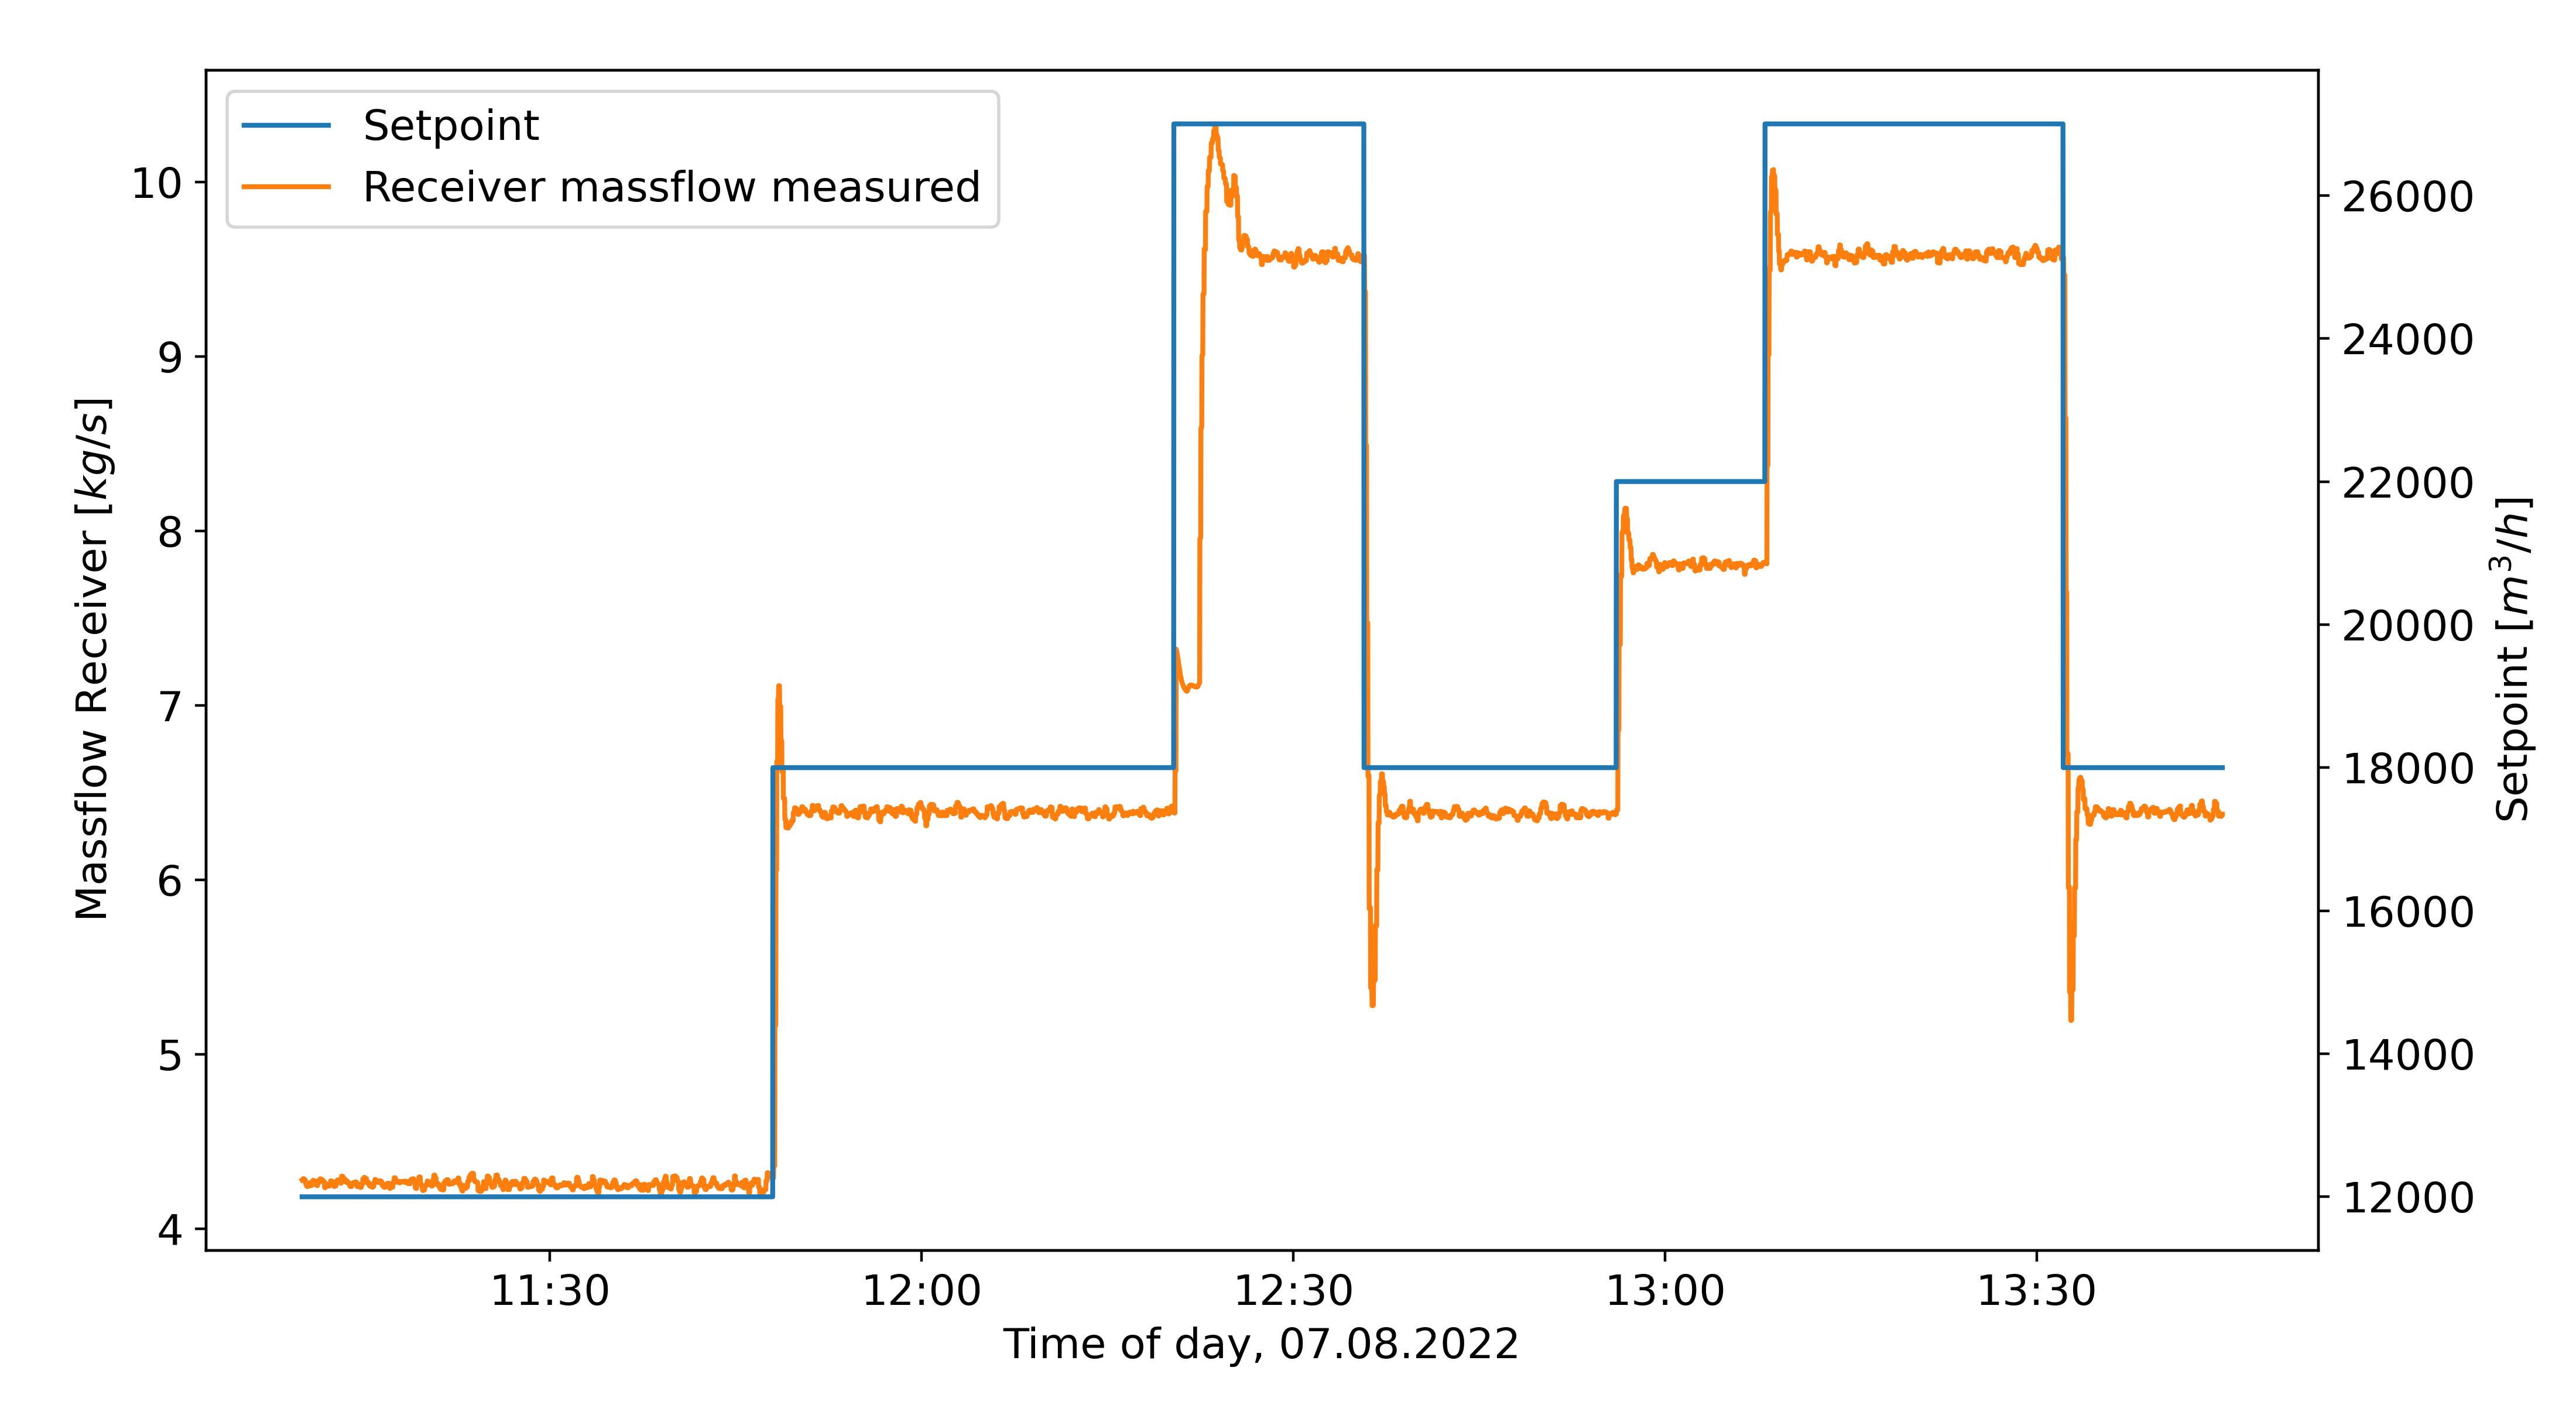
\includegraphics[width=0.95\textwidth]{C:/Users/gesc_ma/VSCode MPC Projekt/dynaovrcontroller/dynaovrcontroller/aimpoint_control_scenarios/plots/12_fan_parameter/measured_fan_data.png}}
    \caption[Luftstrommessung für unterschiedliche Einstellwerte am Solarturm Jülich (07.08.2022)]{Luftstrommessung für unterschiedliche Einstellwerte am Solarturm Jülich (07.08.2022)}
    \label{fig_LuftstromSolarturm}
\end{figure}

Um die Veränderung des Luftmassenstroms bei Einstellwertänderungen simulativ annähern zu können, wird dieser durch ein PT2-Verhalten modelliert.
Die zugehörige Übertragungsfunktion beschreibt das Verhältnis zwischen den Ein- und Ausgangsgrößen, also zwischen dem Einstellwert und dem Massenstrom.
Formel \ref{eq_ÜbertrgaungsfunktionPT2} zeigt die allgemeine Übertragungsfunktion eines schwingungsfähigen PT2-Gliedes als Funktion der Laplace-Variablen $s$ \cite[S.60]{ProfMueller}.

\begin{equation} \label{eq_ÜbertrgaungsfunktionPT2}
    G(s)=\frac{Y(s)}{U(s)}=\frac{K_p}{T^2 \cdot s^2+2 \cdot D \cdot T \cdot s+1}
\end{equation}
% \centerline{\small{\textsf{\textbf{Formel \ref{eq_Label}:}} Beschriftung}}
\myequations{\quad Übertragungsfunktion eines schwingungsfähigen PT2 Gliedes (gemäß \cite[S.60]{ProfMueller})}

Zur Beschreibung des vorliegenden PT2-Verhaltens werden die drei unbekannten Größen der Formel \ref{eq_ÜbertrgaungsfunktionPT2} benötigt.
Dies ist die Zeitkonstante $T$ zur Beschreibung der Geschwindigkeit der Veränderung, die Dämpfungskonstante $D$, die das Einschwingverhalten beschreibt und ein Proportionalitätsfaktor $K_p$.
Anhand der nachfolgenden Abbildung \ref{fig_SprungantwortSymbolisch} werden die Messgrößen einer Einheitssprungantwort $h(t)$ identifiziert, die zur Bestimmung dieser Größen benötigt werden.

\begin{figure}[h!]
    \centering
    \setlength{\fboxsep}{1pt}
    \setlength{\fboxrule}{1pt}
    \fbox{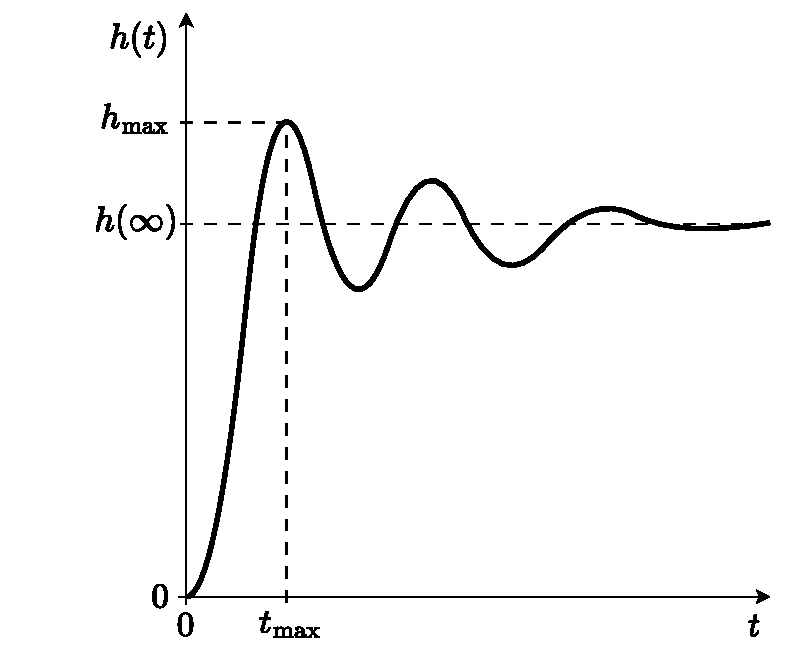
\includegraphics[width=0.55\textwidth]{fig/Sprungantwort}}
    \caption[Exemplarische Einheitssprungantwort eines PT2-Gliedes]{Exemplarische Einheitssprungantwort eines PT2-Gliedes (nach \cite[S.60]{ProfMueller})}
    \label{fig_SprungantwortSymbolisch}
\end{figure}

Der Proportionalitätsfaktor $K_p$ gleicht für eine Einheitssprungantwort dem Wert der von $h(t\rightarrow \infty)$ \cite[S.60]{ProfMueller}.
Grund dafür ist, dass der Einheitssprung eine Veränderung der Eingangsgröße von $0$ auf $1$ impliziert und die Ausgangsgröße vor der Anregung ebenfalls $0$ beträgt.
Allgemein lässt sich $K_p$ nach Gleichung \ref{eq_BerechnungKP} ermitteln.

\begin{equation} \label{eq_BerechnungKP}
    K_p = \frac{h(t\rightarrow \infty) - h(t=0)}{\Delta u}
\end{equation}
% \centerline{\small{\textsf{\textbf{Formel \ref{eq_Label}:}} Beschriftung}}
\myequations{\quad Berechnung des Proportionalitätsfaktors $K_p$ bei PT2-Gliedern}

Für schwingfähige Systeme ergibt sich der Dämpfungsfaktor $D$ aus der relativen Überschwingweite $os$ der Sprungantwort.
Es gilt:
\begin{equation} \label{eq_BerechnungD}
    D = \frac{\ln \left(\frac{1}{os}\right)}{\sqrt{\pi^2+\left(\ln\left[\frac{1}{os}\right]\right)^2}},
\end{equation}
% \centerline{\small{\textsf{\textbf{Formel \ref{eq_Label}:}} Beschriftung}}
\myequations{\quad Berechnung des Dämpfungsfaktors $D$ bei PT2-Gliedern}

\vspace*{-\baselineskip}mit

\begin{equation} \label{eq_overshoot}
    os = \frac{h_{\mathrm{max}}-h(t\rightarrow \infty)}{h(t\rightarrow \infty)}.
\end{equation}
% \centerline{\small{\textsf{\textbf{Formel \ref{eq_Label}:}} Beschriftung}}
\myequations{\quad Berechnung der relativen Überschwingweite $os$}

Die Zeitkonstante eines PT2-Gliedes ergibt sich durch Inbezugnahme des Zeitpunktes $t_{\mathrm{max}}$, zu dem das maximale Überschwingen $h_{\mathrm{max}}$ auftritt (vgl. Abbildung \ref{fig_SprungantwortSymbolisch}).
Sie berechnet sich wie folgt:

\begin{equation} \label{eq_BerechnungT}
    T = \frac{t_{\mathrm{max}} \cdot \sqrt{1-D^2}}{\pi}
\end{equation}
% \centerline{\small{\textsf{\textbf{Formel \ref{eq_Label}:}} Beschriftung}}
\myequations{\quad Berechnung des Dämpfungsfaktors $T$ bei PT2-Gliedern}


\subsection{Mathematische Beschreibung der Lüftungsdynamik}
Unter Betrachtung der verwertbaren Einstellwertänderungen in Abbildung \ref{fig_LuftstromSolarturm} werden die konkreten Parameter der Lüftungsdynamik bestimmt.
Dazu werden die drei Parameter $K_p$, $D$ und $T$ für jeden Eingangssprung errechnet und anschließend gemittelt.
Es ergibt sich \linebreak$K_p = \SI{3.55e-4}{}$, $D = \SI{0.35}{}$ und $T = \SI{11.60}{}$.
Die Plausibilität dieser Berechnungen zeigt nachfolgend Abbildung \ref{fig_LuftstromplusSimulativ}, in der erkennbar ist, dass das simulierte Verhalten des Massenstroms mit den Messwerten übereinstimmt.
Die Wurzel des mittleren quadratischen Fehlers (der \textit{RMSE}) liegt über den Simulationszeitraum unter Ausschluss der invaliden Daten zwischen 12:20 Uhr und 12:40 Uhr bei $\SI{0.043}{\kilo\gram\per\second}$.

\begin{figure}[h!]
    \centering
    \setlength{\fboxsep}{1pt}
    \setlength{\fboxrule}{1pt}
    \fbox{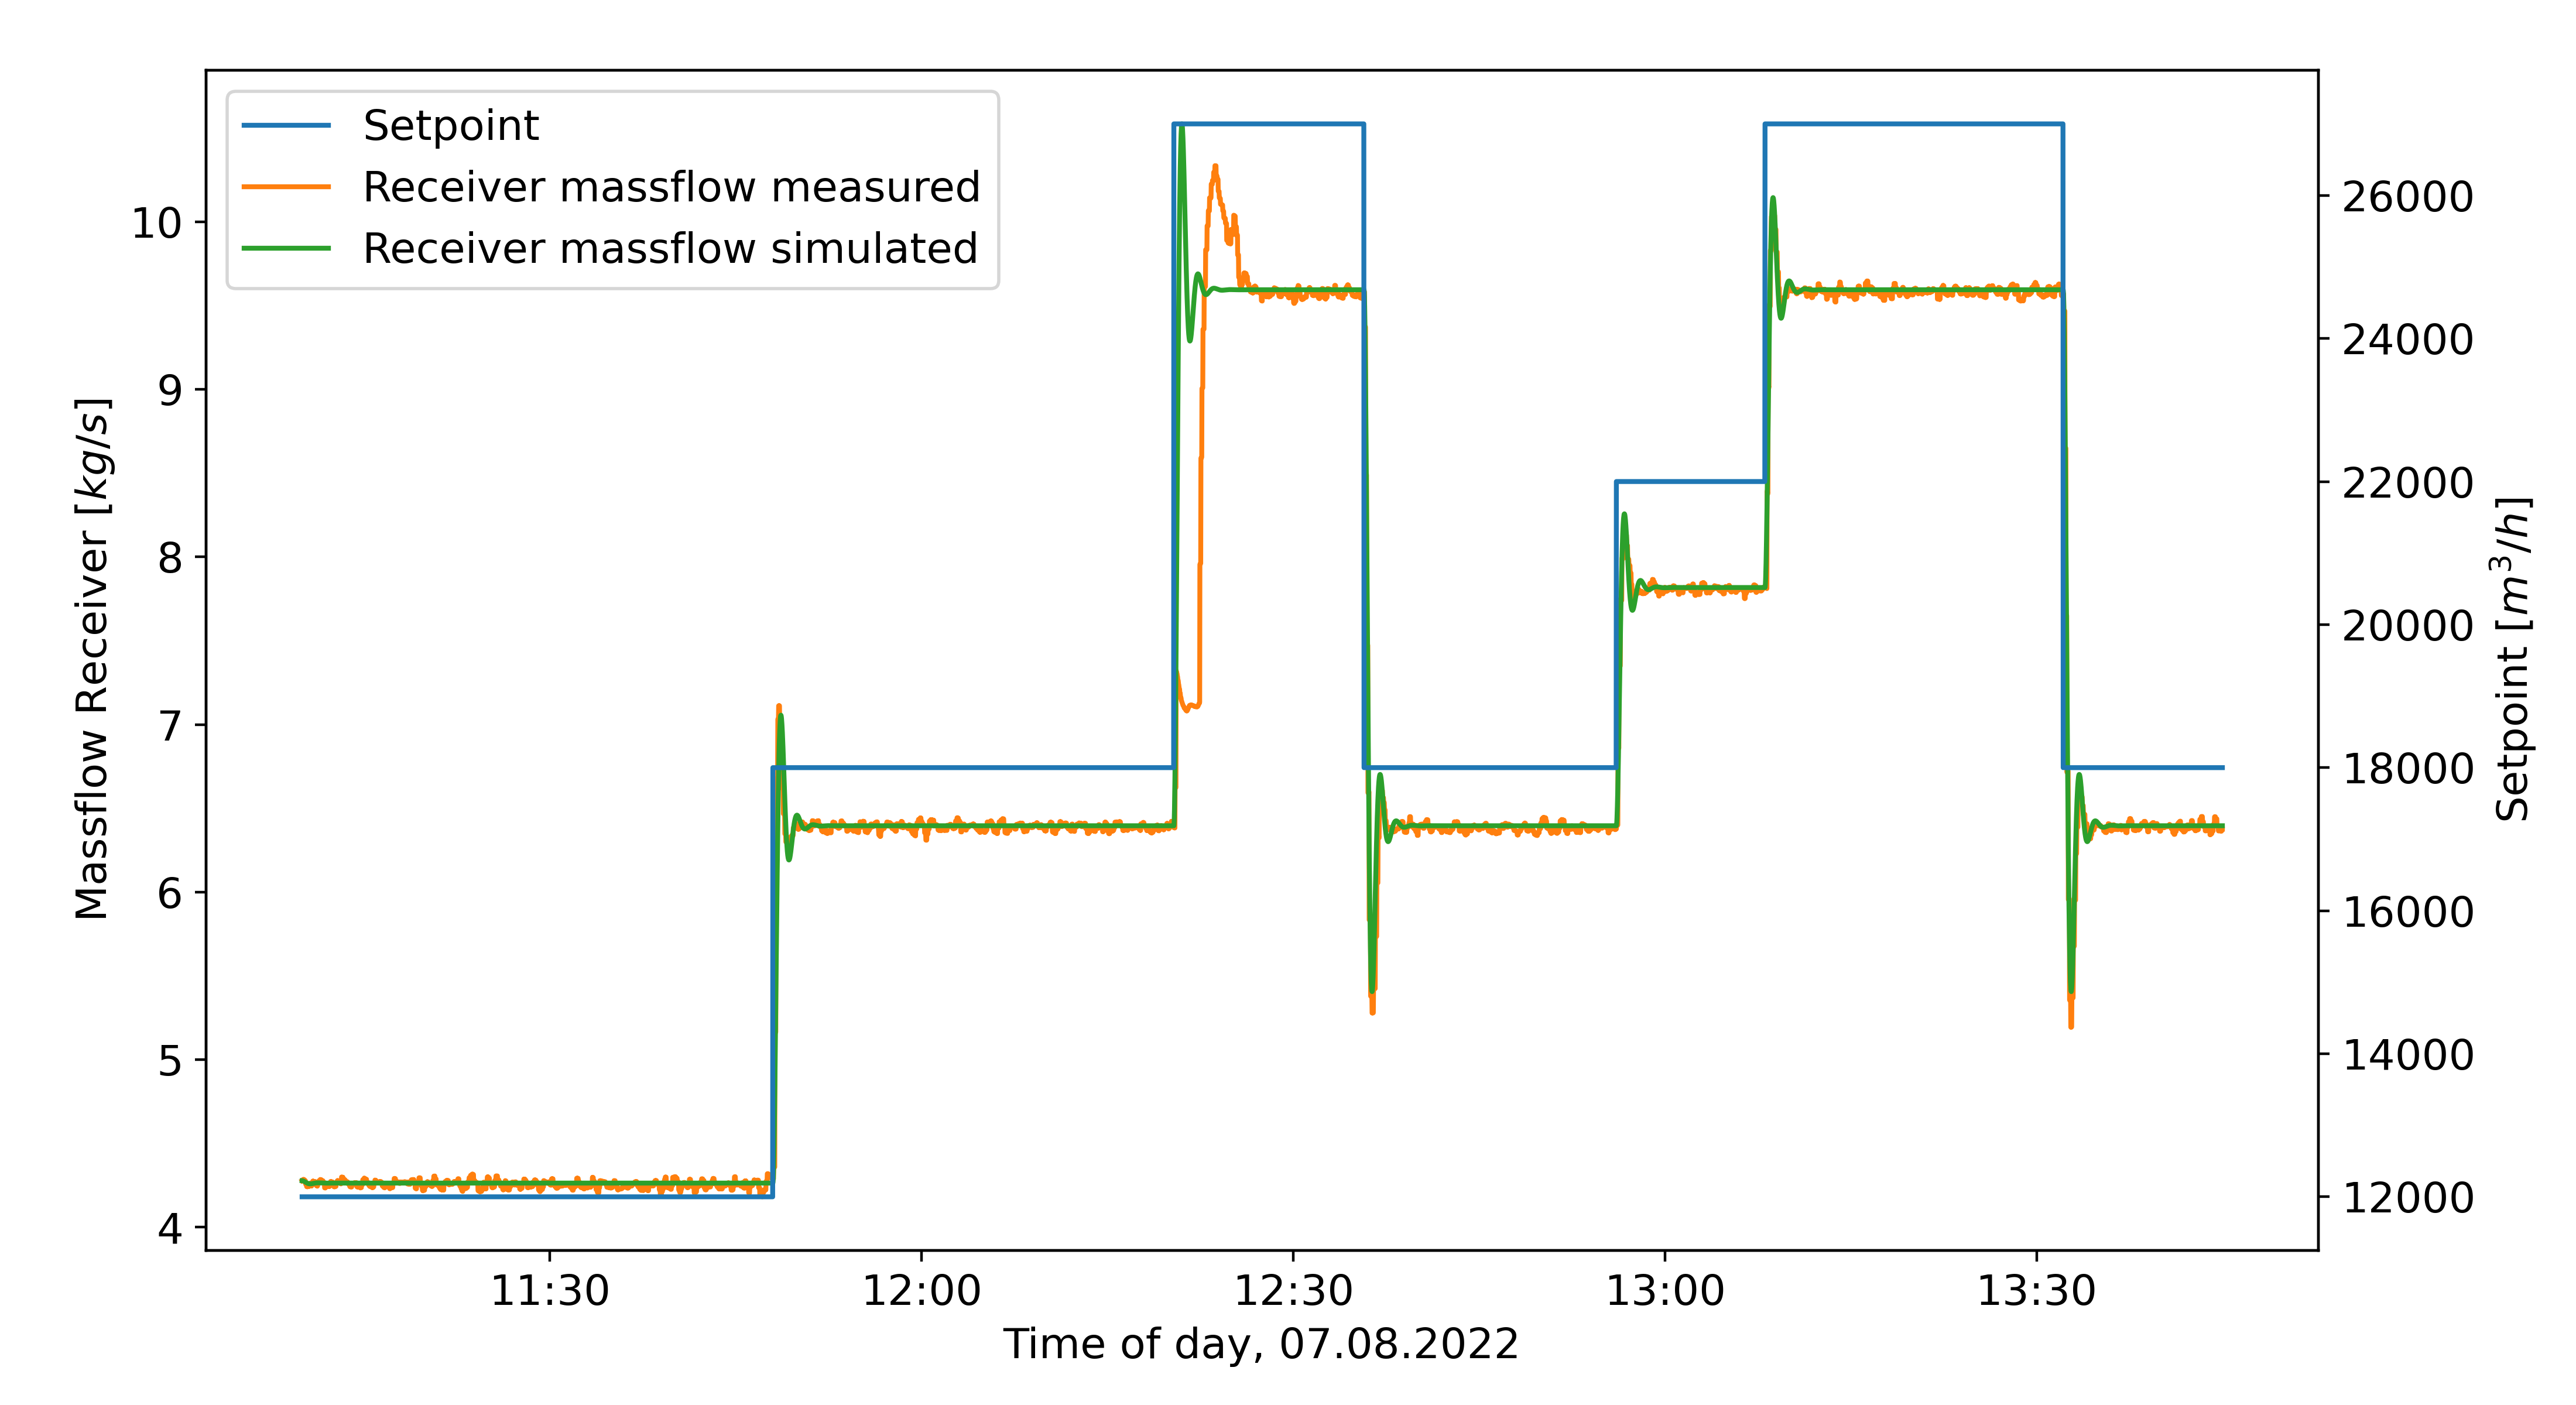
\includegraphics[width=0.95\textwidth]{C:/Users/gesc_ma/VSCode MPC Projekt/dynaovrcontroller/dynaovrcontroller/aimpoint_control_scenarios/plots/12_fan_parameter/fan_parameter_fitting.png}}
    \caption[Vergleich der simulierten Massenströme mit den Messwerten vom 07.08.2022]{Vergleich der simulierten Massenströme mit den Messwerten vom 07.08.2022}
    \label{fig_LuftstromplusSimulativ}
\end{figure}

Im Zeitbereich ergibt sich Gleichung \ref{eq_ÜbertrgaungsfunktionPT2} mit der Ausgangsgröße $Y$ als Luftmassenstrom $\MDotReceiver$ zu der in Gleichung \ref{eq_GesamtDGL} dargestellten Differentialgleichung zweiter Ordnung.
Dabei steht $u_{\mathrm{setpoint}}(t)$ für den zeitlich veränderlichen Einstellwert.

\begin{equation} \label{eq_GesamtDGL}
    K_p \cdot u_{\mathrm{setpoint}}(t) = T^2 \cdot \frac{d^2\MDotReceiver}{dt^2} + 2 \cdot D \cdot T \cdot \frac{d\MDotReceiver}{dt} + \MDotReceiver
\end{equation}
% \centerline{\small{\textsf{\textbf{Formel \ref{eq_Label}:}} Beschriftung}}
\myequations{\quad Differentialgleichung der Lüftungsdynamik}

Aufgrund des geringeren Berechnungsaufwandes bei der numerischen Lösung von Differentialgleichungen erster Ordnung im Vergleich zu solchen mit höherer Ordnung \cite[S.138-139]{Gausch}\cite[S.241ff]{Howell}, wird Gleichung \ref{eq_GesamtDGL} in zwei Differentialgleichungen erster Ordnung umgeschrieben.
Dazu werden zwei Zustände eingeführt; einer für den Massenstrom $\MDotReceiver$ und einer für dessen zeitliche Änderung $\ddot{m}_{\mathrm{rec}}$.
% \begin{equation} \label{eq_Einführtungstates}
%     \begin{gathered}
%         x_1 = \MDotReceiver\\
%         x_2 = \ddot{m}_{\mathrm{rec}}
%     \end{gathered}
% \end{equation}
% % \centerline{\small{\textsf{\textbf{Formel \ref{eq_Label}:}} Beschriftung}}
% \myequations{\quad Einführung des Massenstroms und dessen Ableitung als Systemzustände}
Die erste Differentialgleichung ergibt sich zu:
\begin{equation} \label{eq_ErsteDGLMassflow}
    \frac{d\MDotReceiver}{dt} = \ddot{m}_{\mathrm{rec}}
\end{equation}
% \centerline{\small{\textsf{\textbf{Formel \ref{eq_Label}:}} Beschriftung}}
\myequations{\quad Differentialgleichung zur Beschreibung des Massenstroms}

Aus Gleichung \ref{eq_GesamtDGL} folgt außerdem:
\begin{equation} \label{eq_ZweiteDGLMassflow}
    T^2 \cdot \frac{d\ddot{m}_{\mathrm{rec}}}{dt} = K_p\cdot u_{\mathrm{setpoint}}(t) - 2 \cdot D \cdot T \cdot \ddot{m}_{\mathrm{rec}} - \MDotReceiver
\end{equation}
% \centerline{\small{\textsf{\textbf{Formel \ref{eq_Label}:}} Beschriftung}}
\myequations{\quad Differentialgleichung zur Beschreibung der Massenstromänderung}

Das vollständige thermische Teilmodell ergibt sich durch die Modellierung der Absorbercups nach Kapitel \ref{sec_Ausgangszustand} wobei die ursprüngliche Betrachtung des Massenstroms als Eingangsgröße (vgl. Absatz \ref{subsubsec_Header}) verändert wird.
Durch Einführung des Massenstroms und dessen Ableitung als Systemzustände ist der dimensionslose Einstellfaktor $u_{\mathrm{setpoint}}$ die einzige Eingangsgröße des thermischen Modells.

Der Solarturm in Jülich besteht aus $\SI{36}{} \times \SI{30}{}$ Absorbercups.
Jeder dieser $1080$ Cups wird wie in Kapitel \ref{subsec_ModellCup} erläutert durch zwei Differnzialgleichungen und zwei algebraische Gleichungen beschrieben.
Aufgrund des daraus resultierenden hohen Rechenaufwandes zur Lösung eines Optimierungsproblems dieser Größe wird das thermische Modell auf $\SI{6}{} \times \SI{5}{}$ Cups reduziert.
Dafür werden je $36$ Blendendurchmesser der Absorbercups gemittelt, um den Massenstrom durch einen repräsentativen Cup des jeweiligen Receiverbereiches zu erhalten.
Insgesamt ergibt sich ein System aus $60$ algebraischen Gleichungen und $60+2$ Differentialgleichungen zur Modellierung des thermischen Systems.



\section{Optisches Teilmodell} \label{sec_optischesModell}
% Vorher schon beschrieben und von David hierher gewollt!
Für die Analyse des Systems wird nachfolgend mit vorberechneten Strahlungskarten aus dem in \cite[S.53ff]{DissBelhomme} vorgestellten Programm \textit{STRAL} verwendet.
Die Software berücksichtigt das reale Heliostatenfeld am Standort Jülich und bietet auch die Möglichkeit optische Verluste zu einem gewissen Grad mit einzubeziehen.

% Schon geschrieben: Welchen Regelalgorithmus wähle ich warum?!
Die Algorithmen, die nicht auf Basis einer Gruppierung von Heliostaten funktionieren, haben einen hohen Rechen- und Zeitaufwand in der Optimierung.
Weiterhin ist der DAPS-Algorithmus aufgrund anderer Nachteile für diese Arbeit ungeeignet.
Dazu zählt, dass er nicht für die Inbezugnahme von Wolken ausgelegt ist und keine Leistungsmaximierung geschieht, sondern lediglich die Einhaltung der Grenztemperaturen gewährleistet wird.
Darüber hinaus besteht die Notwendigkeit einer sehr präzisen Modellbildung, um den exakten Einfluss einzelner Heliostaten nutzen zu können.
Weiterhin wird immer der Heliostat mit dem größten Einfluss manipuliert, welcher nicht zwangsläufig der ideale Heliostat in Bezug auf die Optimierung ist \cite[S.35]{DissOberkirsch}.
Die Einteilung des Systems in SISO-Subsysteme ist für stark gekoppelte Systeme mit großen Abhängigkeiten nicht sinnvoll \cite[S.33]{DissZanger}.

% Schon geschrieben: Änderungen an dem Algorithmus
Für die vorliegende Arbeit entfällt die Unterteilung in 18 Gruppen aufgrund der Receiver- und Heliostatenfeldstruktur, sodass das gesamte Feld in lediglich drei Teile eingeteilt wird.
Weiterhin unterscheiden sich in dieser Ausarbeitung auch die erste und zweite Gruppe in der Distanz bezogen auf den Receiver, wie in Kapitel \ref{sec_ErweiterungModellbildung} erläutert wird.


Hier auch hinschreiben, dass linear approximiert wurde

Warum haben wir uns für die Überlagerung der Flussdichtekarten entschieden?
Wie groß ist der prozentuale Fehler durch Vorkalkulation in der Mitte und Verschiebung zum Zielpunkt im Vergleich zur direkten Simulation an der richtigen Stelle?



Alles bezüglich der Heliostaten und deren Gruppierung (Warum 20x20, wegen NowCasting) sowie der Fluxmap 6x5 Verteilung.
Erläutern, dass direktes Mapping auf die Flussdichte nicht funktionieren kann?
Daher Berechnung der Flussdichteverteilung über gruppierte Zielpunktregelung, Wolken können am einfachsten implementiert werden.

Vorberechnete Strahlungskarten verwendet.
Welche Fehler wurden dabei berücksichtigt? David fragen!! (mirror error Prozentsatz etc)


\section{Kopplung der Teilmodelle} \label{sec_KopplungModelle}
Hier muss stehen, dass entsprechend dem optischen Modell 62 Differenzialgleichungen und 60 algebraische Gleichungen das vollständige Modell beschreiben.

% Wichtig:
Modell muss sich in den Details mit dem decken, was der David in seinem Paper mit meinem Namen darauf beschreibt!
Besonders auch, dass die Heliostaten als quasi-statisch anzunehmen sind.
